%iffalse
\let\negmedspace\undefined
\let\negthickspace\undefined
\documentclass[journal,12pt,onecolumn]{IEEEtran}
\usepackage{cite}
\usepackage{amsmath,amssymb,amsfonts,amsthm}
\usepackage{algorithmic}
\usepackage{graphicx}
\usepackage{textcomp}
\usepackage{xcolor}
\usepackage{txfonts}
\usepackage{listings}
\usepackage{enumitem}
\usepackage{mathtools}
\usepackage{gensymb}
\usepackage{comment}
\usepackage[breaklinks=true]{hyperref}
\usepackage{tkz-euclide} 
\usepackage{listings}
\usepackage{gvv}                                        
% \usepackage{gvv}  
\usepackage[latin1] {inputenc}
\usepackage{xparse}
\usepackage{color}                                            
\usepackage{array}                                            
\usepackage{longtable}                                       
\usepackage{calc}                                             
\usepackage{multirow}
\usepackage{multicol}
\usepackage{hhline}                                           
\usepackage{ifthen}                                           
\usepackage{lscape}
\usepackage{tabularx}
\usepackage{array}
\usepackage{float}
\newtheorem{theorem}{Theorem}[section]
\newtheorem{problem}{Problem}
\newtheorem{proposition}{Proposition}[section]
\newtheorem{lemma}{Lemma}[section]
\newtheorem{corollary}[theorem]{Corollary}
\newtheorem{example}{Example}[section]
\newtheorem{definition}[problem]{Definition}
\newcommand{\BEQA}{\begin{eqnarray}}
\newcommand{\EEQA}{\end{eqnarray}}
\usepackage{float}
%\newcommand{\define}{\stackrel{\triangle}{=}}
\theoremstyle{remark}
\usepackage{ circuitikz }
%\newtheorem{rem}{Remark}
% Marks the beginning of the document
\begin{document}
\title{GATE BT 2025}
\author{EE25BTECH11044 - Pappula Sai Hasini}
\maketitle
\renewcommand{\thefigure}{\theenumi}
\renewcommand{\thetable}{\theenumi}
%GATE BT 2025
\begin{enumerate}
\item
If `$\rightarrow$` denotes increasing order of intensity, then the meaning of the words [dry $\rightarrow$ arid $\rightarrow$ parched] is analogous to [diet $\rightarrow$ fast $\rightarrow$ \_\_\_\_\_\_]. Which one of the given options is appropriate to fill the blank?
\begin{enumerate}
   \item starve 
   \item reject 
   \item feast 
   \item deny 
\end{enumerate}
\hfill(GATE BT 2025)


\item 
If two distinct non-zero real variables $x$ and $y$ are such that $x+y \propto x-y$, then the value of $x/y$ is

\begin{enumerate}
    \item depends on $xy$
    \item depends only on $x$ and not on $y$
    \item depends only on $y$ and not on $x$
    \item is a constant
\end{enumerate}
\hfill(GATE BT 2025)

\item 
Consider the following sample of numbers: $9, 18, 11, 14, 15, 17, 10, 69, 11, 13$. The median of the sample is

\begin{enumerate}
    \item $13.5$
    \item $14$
    \item $11$
    \item $18.7$
\end{enumerate}
\hfill(GATE BT 2025)

\item The number of coins of Rs.~1, Rs.~5, and Rs.~10 denominations that a person has are in the ratio $5:3:13$. Of the total amount, the percentage of money in Rs.~5 coins is \_\_\_.

\hfill (GATE BT 2025)


\begin{enumerate}
    \item $21\%$
    \item $14\%$
    \item $10\%$
    \item $30\%$
\end{enumerate}
\hfill(GATE BT 2025)

\item 
For positive non-zero real variables $p$ and $q$, if $\log(p^2+q^2)=\log p+\log q+2\log 3$, then the value of $\dfrac{p^4+q^4}{p^2 q^2}$ is

\begin{enumerate}
    \item $79$
    \item $81$
    \item $9$
    \item $83$
\end{enumerate}
\hfill(GATE BT 2025)

\item 
In the given text, the blanks are numbered (i)(iv). Select the best match for all the blanks. 

Steve was advised to keep his head (i) before heading (ii) to bat; for, while he had a head (iii) batting, he could only do so with a cool head (iv) his shoulders. 

\begin{enumerate}
    \item (i) down (ii) down (iii) on (iv) for
    \item (i) on (ii) down (iii) for  (iv) on
    \item (i) down (ii) out (iii) for (iv) on
    \item (i) on (ii) out  (iii) on (iv) for
\end{enumerate}
\hfill(GATE BT 2025)

\item 
A rectangular paper sheet of dimensions $54\,\text{cm} \times 4\,\text{cm}$ is taken. The two longer edges of the sheet are joined together to create a cylindrical tube. A cube whose surface area is equal to the area of the sheet is also taken. Then, the ratio of the volume of the cylindrical tube to the volume of the cube is

\begin{enumerate}
    \item $1/\pi$
    \item $2/\pi$
    \item $3/\pi$
    \item $4/\pi$
\end{enumerate}
\hfill(GATE BT 2025)

\item The least number of squares to be added in the figure to make $AB$ a line of symmetry is

\begin{center}
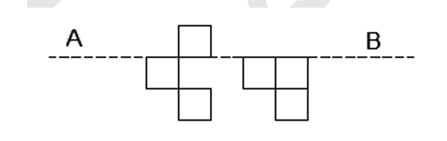
\includegraphics[width=\columnwidth]{figs/figure_path.png}
\label{fig:figure_path}
\end{center}

\begin{enumerate}
    \item 6
    \item 4
    \item 5
    \item 7
\end{enumerate}

\item 
A rectangular paper of $20\,\text{cm} \times 8\,\text{cm}$ is folded $3$ times. Each fold is made along the line of symmetry, which is perpendicular to its long edge. The perimeter of the final folded sheet (in cm) is

\begin{enumerate}
    \item $18$
    \item $24$
    \item $20$
    \item $21$
\end{enumerate}
\hfill(GATE BT 2025)

\item 
In adsorption chromatography, the adsorption of uncharged solute molecules onto a silica-based stationary phase is by \_\_\_\_\_\_.

\begin{enumerate}
    \item covalent bonds
    \item electrostatic interactions
    \item ionic bonds
    \item van der Waals forces
\end{enumerate}
\hfill(GATE BT 2025)

\item 
The total fat (all three types), in grams, this person consumes is
\begin{center}
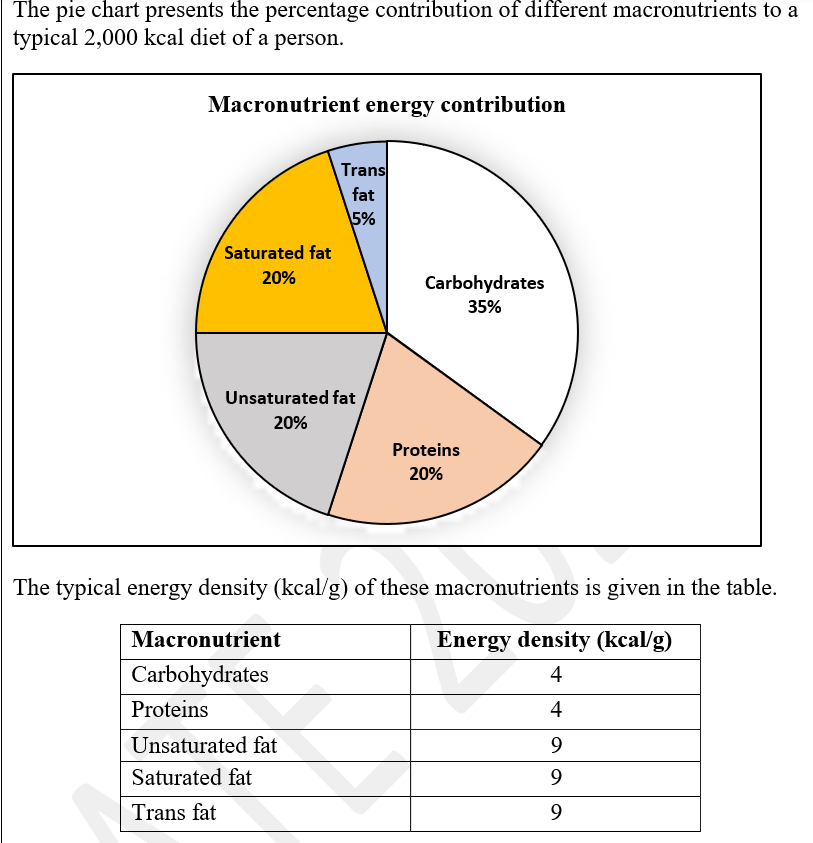
\includegraphics[width=\columnwidth]{figs/table.png}
    \label{fig:macronutrient_pie}
\end{center}

\item 
The transfer function of a process is $G(s) = \dfrac{K_p}{\tau_p s + 1}$, where $K_p$ is the gain and $\tau_p$ is the time constant. This is a \_\_\_\_\_\_ process.

\begin{enumerate}
    \item first order
    \item multi-capacity
    \item purely capacitive
    \item second order
\end{enumerate}
\hfill(GATE BT 2025)

\item 
Which one of the following statements is correct in the context of thermodynamics?

\begin{enumerate}
    \item In a closed system, neither mass nor energy is transferred across the system boundary
    \item In a closed system, both mass and energy can be transferred across the system boundary
    \item The total energy of the system is the sum of kinetic and potential energies
    \item In a closed system, only energy can be transferred across the system boundary and not mass
\end{enumerate}
\hfill(GATE BT 2025)

\item 
Which one of the following statements is correct about Reynolds Number ($N_{Re}$) in a stirred tank bioreactor?

\begin{enumerate}
    \item $N_{Re}$ is independent of the viscosity of the medium
    \item In laminar flow, mixing time increases with an increase in $N_{Re}$
    \item $N_{Re}$ is inversely proportional to the impeller speed
    \item In turbulent flow, mixing time is independent of $N_{Re}$
\end{enumerate}
\hfill(GATE BT 2025)

\item 
The relationship that involves the exchange of nutrients between two different species for their mutual growth is called \_\_\_\_\_\_.

\begin{enumerate}
    \item antagonism
    \item commensalism
    \item parasitism
    \item syntrophism
\end{enumerate}
\hfill(GATE BT 2025)

\item 
Mendels law of segregation applies to the segregation of \_\_\_\_\_\_ during gamete formation.

\begin{enumerate}
    \item mitochondrial genes
    \item alleles of a gene
    \item linked genes on the same chromosome
    \item unlinked genes on the same chromosome
\end{enumerate}
\hfill(GATE BT 2025)

\item 
Co-translational translocation of proteins is observed in \_\_\_\_\_\_.

\begin{enumerate}
    \item endoplasmic reticulum
    \item Golgi complex
    \item mitochondria
    \item peroxisomes
\end{enumerate}
\hfill(GATE BT 2025)

\item 
2-mercaptoethanol breaks the \_\_\_\_\_\_ covalent bond between light and heavy chains of an immunoglobulin molecule.

\begin{enumerate}
    \item C-N
    \item N-O
    \item S-C
    \item S-S
\end{enumerate}
\hfill(GATE BT 2025)

\item 
During normal embryonic development of the mice paw, elimination of cells from the inter-digital space is due to \_\_\_\_\_\_.

\begin{enumerate}
    \item apoptosis
    \item meiosis
    \item mutagenesis
    \item necrosis
\end{enumerate}
\hfill(GATE BT 2025)

\item 
A cultured skin fibroblast cell of a goat P was fused with an enucleated ovum of a goat Q. The resultant activated early embryo was then transplanted into a pseudopregnant (surrogate) female goat R of the same strain as Q. On completion of gestation, a female goat S was born. With the exception of mitochondrial DNA, S is a clone of \_\_\_\_\_\_.

\begin{enumerate}
    \item Only P
    \item Only Q
    \item Only R
    \item Both P and R
\end{enumerate}
\hfill(GATE BT 2025)

\item 
Which one of the following bacteriophages has a genome composed of single stranded circular DNA?

\begin{enumerate}
    \item $\phi$X174
    \item $\lambda$
    \item T5
    \item P1
\end{enumerate}
\hfill(GATE BT 2025)

\item 
Which one of the following is an insect cell line?

\begin{enumerate}
    \item HEK 293
    \item Sf9
    \item DH5$\alpha$
    \item CHO
\end{enumerate}
\hfill(GATE BT 2025)

\item 
Which one of the following is the basic principle of Sangers DNA sequencing method?

\begin{enumerate}
    \item Chain termination by incorporation of dideoxynucleotides
    \item Chain elongation by incorporation of dideoxynucleotides
    \item Release of inorganic pyrophosphate
    \item Chain cleavage by modification of dideoxynucleotides
\end{enumerate}
\hfill(GATE BT 2025)

\item 
An element that is present in a nucleotide but not in a nucleoside is \_\_\_\_\_\_.

\begin{enumerate}
    \item carbon
    \item nitrogen
    \item oxygen
    \item phosphorus
\end{enumerate}
\hfill(GATE BT 2025)

\item 
Krebs (TCA) cycle is \_\_\_\_\_\_ pathway.

\begin{enumerate}
    \item only an anabolic
    \item only a catabolic
    \item an amphibolic
    \item a pyogenic
\end{enumerate}
\hfill(GATE BT 2025)

\item 
If a denatured protein of human origin is injected into a rabbit, antibodies generated will recognize the \_\_\_\_\_\_ structure of the protein.

\begin{enumerate}
    \item primary
    \item secondary
    \item tertiary
    \item quaternary
\end{enumerate}
\hfill(GATE BT 2025)

\item 
All pseudogenes DO NOT code for a \_\_\_\_\_\_.

\begin{enumerate}
    \item protein with original function
    \item protein with altered function
    \item RNA with coding sequence
    \item RNA with regulatory function
\end{enumerate}
\hfill(GATE BT 2025)

\item 
A value of $k$ for which the linear equations $(k-1)x+3y=0$ and $2x+ky=0$ have a non-zero solution is \_\_\_\_\_\_.

\begin{enumerate}
    \item $1$
    \item $2$
    \item $3$
    \item $4$
\end{enumerate}
\hfill(GATE BT 2025)

\item 
The value of the series $1+\sin x+\cos 2x+\sin 3x+\cdots$ at $x=\pi/4$ is \_\_\_\_\_\_.

\begin{enumerate}
    \item $\dfrac{1}{\sqrt{2}+1}$
    \item $\dfrac{\sqrt{2}}{\sqrt{2}+1}$
    \item $\dfrac{1}{\sqrt{2}-1}$
    \item $\dfrac{\sqrt{2}}{\sqrt{2}-1}$
\end{enumerate}
\hfill(GATE BT 2025)

\item 
The solution of the differential equation $\dfrac{dy}{dx}=y+e^{-x}$ that satisfies $y(0)=-\dfrac{1}{2}$ is \_\_\_\_\_\_.

\begin{enumerate}
    \item $-\dfrac{1}{2}e^{-x/2}$
    \item $-\dfrac{1}{2}e^{x}$
    \item $-\dfrac{1}{2}e^{-x}$
    \item $-\dfrac{1}{2}e^{x/2}$
\end{enumerate}
\hfill(GATE BT 2025)

\item 
The six faces of a cube (die) are numbered as $1, 2, 3, 4, 5,$ and $6$, and it is rolled once. An outcome is the observed number on the top face. If the probability of getting an odd number as an outcome is twice that of an even number, then the probability of getting a number less than $3$ is \_\_\_\_\_\_.

\begin{enumerate}
    \item $\dfrac{1}{9}$
    \item $\dfrac{2}{9}$
    \item $\dfrac{1}{3}$
    \item $\dfrac{4}{9}$
\end{enumerate}
\hfill(GATE BT 2025)

\item 
Let $\vec{OR}$ be the vector that is perpendicular to the vectors $\vec{OP}=2\hat{i}-3\hat{j}+\hat{k}$ and $\vec{OQ}=-2\hat{i}+\hat{j}+\hat{k}$. If the length of the vector $\vec{OR}$ is $\alpha\sqrt{3}$, then $\alpha$ is \_\_\_\_\_\_.

\begin{enumerate}
    \item $3$
    \item $4$
    \item $5$
    \item $6$
\end{enumerate}
\hfill(GATE BT 2025)

\item 
The degree of reduction (reductance) for oxalic acid $C_2H_2O_4$ is \_\_\_\_\_\_.

\hfill(GATE BT 2025)

\item 
If the rate at which E. coli divides is $0.5\,\text{h}^{-1}$, then its doubling time is \_\_\_\_\_\_ h.

\hfill(GATE BT 2025)

\item 
The decimal reduction time of a microbe during sterilization at $120^\circ\text{C}$ with a first order thermal death rate constant of $1\,\text{min}^{-1}$ will be \_\_\_\_\_\_ min (rounded off to $1$ decimal place).

\hfill(GATE BT 2025)

\item 
Match the disease (Column I) with its biological vector (Column II).

\begin{tabular}{ll}
Column I & Column II \\
P. Chagas disease & 1. Tsetse flies \\
Q. Trypanosomiasis & 2. Mosquitoes \\
R. Leishmaniasis & 3. Sandflies \\
S. Yellow Fever & 4. Reduviid bugs \\
\end{tabular}

\begin{enumerate}
    \item P-4; Q-1; R-3; S-2
    \item P-2; Q-3; R-4; S-1
    \item P-1; Q-4; R-3; S-2
    \item P-3; Q-1; R-2; S-4
\end{enumerate}
\hfill(GATE BT 2025)

\item Match the industrial enzyme (Column I) with its application (Column II).

\begin{tabular}{ll}
Column I & Column II \\
P. Lipase & 1. Maltose syrup production \\
Q. Ficin & 2. Oil degradation \\
R. Amylase & 3. Oligosaccharide/monosaccharide production \\
S. Glucosidase & 4. Meat tenderization \\
\end{tabular}

\begin{enumerate}
    \item  P-3; Q-4; R-2; S-1 
    \item  P-2; Q-4; R-1; S-3 
    \item  P-2; Q-3; R-1; S-4 
    \item  P-1; Q-2; R-4; S-3
\end{enumerate}
\hfill (GATE BT 2025)

\item Match the enzyme (Column I) with its corresponding function (Column II).

\begin{tabular}{ll}
Column I & Column II \\
P. Primase & 1. RNA dependent RNA synthesis \\
Q. Reverse transcriptase & 2. DNA dependent DNA synthesis \\
R. RNA Replicase & 3. RNA dependent DNA synthesis \\
S. DNA Polymerase III & 4. DNA dependent RNA synthesis \\
\end{tabular}

\begin{enumerate}
\item P-4; Q-1; R-3; S-2 \hfill
\item P-2; Q-1; R-3; S-4 \hfill
\item P-3; Q-4; R-2; S-1 \hfill
\item P-4; Q-3; R-1; S-2
\end{enumerate}

\hfill (GATE BT 2025)

\item Match the item (Column I) with its corresponding use (Column II).

\begin{tabular}{ll}
Column I & Column II \\
P. Glutamine & 1. Detachment of adherent cells \\
Q. Trypsin & 2. Selection of transfected mammalian cell lines \\
R. Hypoxanthine & 3. Source of carbon and nitrogen in animal cell culture media \\
S. Neomycin & 4. A component of medium for selection of hybridoma in monoclonal antibody production \\
\end{tabular}

\begin{enumerate}
\item P-3; Q-1; R-4; S-2 \hfill
\item P-1; Q-2; R-4; S-3 \hfill
\item P-3; Q-1; R-2; S-4 \hfill
\item P-2; Q-3; R-1; S-4
\end{enumerate}

\hfill (GATE BT 2025)

\item Match the chemical (Column I) with its use (Column II).

\begin{tabular}{ll}
Column I & Column II \\
P. Diethylpyrocarbonate & 1. Chelation of magnesium ion during DNA purification \\
Q. Cesium chloride & 2. Prevention of RNA degradation in aqueous environment \\
R. Ethidium bromide & 3. Separation of DNA by density gradient centrifugation \\
S. Ethylenediaminetetraacetic acid & 4. Staining of RNA in agarose gel \\
\end{tabular}

\begin{enumerate}
\item P-4; Q-1; R-3; S-2 \hfill
\item P-4; Q-3; R-2; S-1 \hfill
\item P-2; Q-1; R-4; S-3 \hfill
\item P-2; Q-3; R-4; S-1
\end{enumerate}

\hfill (GATE BT 2025)

\item Match the item in Column I with the corresponding technique in Column II.

\begin{tabular}{ll}
Column I & Column II \\
P. Blue laser & 1. Electron microscopy \\
Q. Tungsten filament & 2. Fluorescence activated cell sorting \\
R. $^{15}$N labelled protein & 3. Electrophoresis \\
S. Polyacrylamide & 4. Nuclear magnetic resonance spectroscopy \\
\end{tabular}

\begin{enumerate}
\item P-2; Q-3; R-1; S-4 \hfill
\item P-2; Q-1; R-4; S-3 \hfill
\item P-3; Q-1; R-4; S-2 \hfill
\item P-1; Q-2; R-4; S-3
\end{enumerate}

\hfill (GATE BT 2025)

\item Match the genetic disorder (Column I) with its molecular basis (Column II).

\begin{tabular}{ll}
Column I & Column II \\
P. Sickle-cell anemia & 1. Mutation in nucleotide excision repair \\
Q. Xeroderma pigmentosum & 2. Trisomy of chromosome 21 \\
R. Tay-Sachs disease & 3. Mutation in $\beta$-globin gene \\
S. Down Syndrome & 4. Mutation in hexosaminidase A gene \\
\end{tabular}

\begin{enumerate}
\item P-1; Q-4; R-2; S-3 \hfill
\item P-3; Q-4; R-1; S-2 \hfill
\item P-3; Q-1; R-4; S-2 \hfill
\item P-4; Q-2; R-3; S-1
\end{enumerate}

\hfill (GATE BT 2025)

\item The evolution of wings in bats and insects is an example of \_\_\_\_\_\_ evolution.

\begin{enumerate}
\item convergent \hfill
\item divergent \hfill
\item neutral \hfill
\item parallel
\end{enumerate}

\hfill (GATE BT 2025)

\item Which of the following statements is/are correct about an uncompetitive inhibitor of an enzyme?

\begin{enumerate}
\item It binds to the substrate binding site of the enzyme only \hfill
\item It binds to the enzyme-substrate complex only \hfill
\item It reduces the Vmax of the enzyme \hfill
\item It binds to both free enzyme and enzyme-substrate complex
\end{enumerate}

\hfill (GATE BT 2025)

\item Which of the following plant-based secondary metabolites belong(s) to the class of alkaloids?

\begin{enumerate}
\item Ajmalicine (C$_{21}$H$_{24}$N$_2$O$_3$) \hfill
\item Azadirachtin (C$_{35}$H$_{44}$O$_{16}$) \hfill
\item Camptothecin (C$_{20}$H$_{16}$N$_2$O$_4$) \hfill
\item Vinblastine (C$_{46}$H$_{58}$N$_4$O$_9$)
\end{enumerate}

\hfill (GATE BT 2025)

\item Which of the following features help(s) in distinguishing alleles using restriction fragment length polymorphism (RFLP)?

\begin{enumerate}
\item Differences in the number of recognition sites for a given restriction enzyme \hfill
\item Differences in the ability of alleles to undergo recombination \hfill
\item Differences in the ability of alleles to undergo segregation \hfill
\item Differences in the number of tandem repeats
\end{enumerate}

\hfill (GATE BT 2025)

\item Which of the following is/are considered as biotic elicitor(s) in plant cell culture?

\begin{enumerate}
\item Cellulase 
\item Chitin 
\item Chitosan 
\item Mercuric chloride
\end{enumerate}

\hfill (GATE BT 2025)

\item Under which of the following conditions, a mammalian somatic cell fails to undergo mitosis during cell cycle?

\begin{enumerate}
\item Initiation of cell plate formation 
\item Incomplete DNA replication 
\item Chiasmata formation 
\item Irreparable DNA damage
\end{enumerate}

\hfill (GATE BT 2025)

\item Which of the following is/are synthetic auxin(s) that does/do NOT occur naturally?

\begin{enumerate}
\item 2,4-Dichlorophenoxyacetic acid 
\item Indole-3-acetic acid 
\item Indole-3-butyric acid 
\item 1-Naphthaleneacetic acid
\end{enumerate}

\hfill (GATE BT 2025)

\item Which of the following statements regarding the below mentioned mRNA sequence is/are TRUE? 

\[
5^\prime-UGAUGAGCCUUAACCGGGAACGAAUUUAAG-3^\prime
\]

\begin{enumerate}
\item It contains nine codons in the reading frame \hfill
\item It contains ten codons in the reading frame \hfill
\item It codes for eight amino acids \hfill
\item It codes for nine amino acids
\end{enumerate}

\hfill (GATE BT 2025)

\item Which of the following conditions induce(s) the expression of $\beta$-galactosidase gene in the lac operon?

\begin{enumerate}
\item Absence of glucose 
\item Absence of lactose 
\item Presence of glucose 
\item Presence of lactose
\end{enumerate}

\hfill (GATE BT 2025)

\item Which of the following factors can affect the growth of a microbial culture in a batch cultivation process?

\begin{enumerate}
\item pH of the medium 
\item Osmolarity of the medium 
\item Substrate concentration in the medium 
\item Substrate feed rate
\end{enumerate}

\hfill (GATE BT 2025)

\item Under complete cell washout condition in a chemostat with sterile feed, which of the following statements is/are correct?  

\begin{enumerate}
    \item Biomass concentration in the reactor is maximum  
    \item Substrate concentration in the exit stream is less than that in the inlet stream  
    \item Substrate concentration in the exit stream is equal to that in the inlet stream  
    \item Substrate concentration in the exit stream is zero  
\end{enumerate}

\hfill (GATE BT 2025)

\item Fermentation medium is cooled from $121^\circ$C to $30^\circ$C in a double pipe heat exchanger. If cold water is flowing in the counter-current direction and is heated from $10^\circ$C to $70^\circ$C, then the Log-Mean Temperature Difference (LMTD) is \_\_\_\_\_\_ $^\circ$C (rounded off to the nearest integer).

\hfill (GATE BT 2025)

\item
Aspergillus niger is grown in a 10,000 L stirred batch bioreactor under aerated conditions to produce citric acid. At steady state oxygen transfer conditions, the specific oxygen uptake rate of the organism and the volumetric mass transfer coefficient are $1\times10^{-4}$ g oxygen consumed g$^{-1}$ biomass s$^{-1}$ and $60$ min$^{-1}$, respectively. If the oxygen solubility is $8\times10^{-3}$ kg m$^{-3}$ under the operating conditions, based only on oxygen dynamics, the maximum possible cell concentration is \_\_\_\_ kg m$^{-3}$ (Answer in integer).
\hfill (GATE BT 2025)

\item Ethanol is produced in a 10{,}000 L stirred bioreactor using an impeller of diameter 1 m. The density and viscosity of fermentation broth are 1000 kg m$^{-3}$ and 1 cP, respectively. The data relating the Power number and Impeller Reynolds number are:

\begin{center}
\begin{tabular}{lccc}
\hline
Reynolds number & 1--5 & 5--500 & $> 10^5$ \\
Power number & 70 & 10 & 5 \\
\hline
\end{tabular}
\end{center}

Using the above data, the power required for the stirrer to operate at 300 rpm is \_\_\_\_\_ kW (Answer in integer).

\hfill (GATE BT 2025)

\item The free energy change of ATP hydrolysis at $25^\circ$C is $-32.2$ kJ mol$^{-1}$. The free energy change for hydrolysis of $\alpha$-glycerophosphate to glycerol is $-8.2$ kJ mol$^{-1}$ at $25^\circ$C. Using the above information, the free energy change for the formation of $\alpha$-glycerophosphate from glycerol and ATP is \_\_\_\_\_\_ kJ mol$^{-1}$ (Answer in integer).

\hfill (GATE BT 2025)

\item \textit{E. coli} is inoculated in a shake flask containing nutrient rich medium. The initial number of viable cells in the medium is $10^2$. After few hours, the number of viable cells is $10^6$. Assuming cell divides by binary fission, the number of generations that have taken place is \_\_\_\_ (rounded off to the nearest integer).

\hfill (GATE BT 2025)

\item A fermentor is filled with medium at a rate of 1 L min$^{-1}$. A leak develops at the bottom of the fermentor when the medium in the fermentor reaches 200 L. The rate of medium leakage is $2t$ L min$^{-1}$, where $t$ is the time (in minutes) from when the leak begins. The volume of medium in the fermentor after 10 min of leakage is \_\_\_\_\_ L (Answer in integer).

\hfill (GATE BT 2025)

\item A fed batch process is running at quasi-steady state with respect to substrate and biomass concentration. At 2 h, the culture volume is 500 L with a constant sterile inlet feed at 50 L h$^{-1}$ of glucose. The culture kinetic parameters $\mu_m$ and $K_S$ are 0.2 h$^{-1}$ and 0.1 g L$^{-1}$, respectively. The substrate concentration in the reactor will be \_\_\_\_\_ g L$^{-1}$ (rounded off to one decimal place).

\hfill (GATE BT 2025)

\item Consider scale-up of fungal fermentation from a 20 L model-type to 20{,}000 L prototype stirred tank reactor. The model-type and prototype have the same aspect ratio during scale-up. The impeller speed in the model-type is 500 rpm and the scale-up criterion is constant shear. The impeller speed in the prototype reactor will be \_\_\_\_\_ rpm (Answer in integer).

\hfill (GATE BT 2025)

\item If $\vec{v}=\begin{pmatrix}2\\[2pt]1\\[2pt]2\end{pmatrix}$ is an eigenvector of the matrix
$\begin{pmatrix}
1 & 2 & 3\\
2 & 1 & 2\\
3 & 2 & 1
\end{pmatrix}$ corresponding to the non-zero eigenvalue $\lambda$, then the value of $\lambda$ is \_\_\_.

\hfill (GATE BT 2025)

\item The value of the limit $\displaystyle \lim_{x\to\infty} x\ln\!\left(1+\frac{2}{x}\right)$ is \_\_\_.

\hfill (GATE BT 2025)

\item Let $y(x)=x^2\ln x$ for $x>0$ be a solution of
\[
x^2\frac{d^2 y}{dx^2}+4y=\alpha x\frac{dy}{dx}.
\]
Then the value of $\alpha$ is \_\_\_.

\hfill (GATE BT 2025)

\item The absolute relative error in evaluating the integral $\displaystyle \int_{0}^{1} x^2\,dx$ by the trapezoidal rule with the step size $0.25$ is \_\_\_% (rounded off to 2 decimal places).

\hfill (GATE BT 2025)

\end{enumerate}
\end{document}